%\documentclass[12pt,pdftex,aos]{imsart}
\documentclass[12pt,pdftex,generic]{imsart}

\RequirePackage[OT1]{fontenc}
\usepackage{amsthm,amsmath,amsfonts,natbib,mathtools}
\RequirePackage{hypernat}
\usepackage[ruled,section]{algorithm}
\usepackage[noend]{algorithmic}
\usepackage{graphicx}
\usepackage[hscale=0.7,vscale=0.8]{geometry}
\usepackage{subfigure}
\usepackage{graphicx}
\usepackage{hyperref}
\usepackage{yhmath}
\usepackage{accents}


\renewcommand{\baselinestretch}{1.1}
%\parskip12pt
%\parindent0pt
\setcounter{tocdepth}{2}

\newcommand{\fix}{\marginpar{FIX}}
\newcommand{\new}{\marginpar{NEW}}
\DeclareMathOperator{\rank}{rank}
\DeclareMathOperator{\diag}{diag}
\DeclareMathOperator{\trace}{trace}
\DeclareMathOperator{\pr}{Prob}
\DeclareMathOperator{\cov}{Cov}
\newcommand{\EE}[1]{\mathbb{E}({#1})}
\def\interleave{|\kern-.25ex|\kern-.25ex|}
\def\interleavesub{|\kern-.15ex|\kern-.15ex|}
\newcommand{\nnorm}[1]{\interleave {#1} \interleave}
\newcommand{\nnormsub}[1]{\interleavesub {#1} \interleavesub}
\newcommand{\nNorm}[1]{\left|\kern-.25ex\left|\kern-.25ex\left| {#1}\right|\kern-.25ex\right|\kern-.25ex\right|}
\newcommand{\norm}[1]{\left\|{#1}\right\|}
%\newcommand{\trnorm}[1]{\norm{{#1}}_{\mathrm{tr}}}
\newcommand{\trnorm}[1]{\norm{{#1}}_{*}}
\newcommand{\spnorm}[1]{\norm{{#1}}_{\mathrm{sp}}}
\newcommand{\frnorm}[1]{\norm{{#1}}_{\mathrm{F}}}
%\newcommand{\trnnorm}[1]{\nnorm{{#1}}_{\mathrm{tr}}}
\newcommand{\trnnorm}[1]{\nnorm{{#1}}_{*}}
\newcommand{\spnnorm}[1]{\nnorm{{#1}}_{\mathrm{sp}}}
\newcommand{\spnnormsub}[1]{\nnormsub{{#1}}_{\mathrm{sp}}}
\newcommand{\frnnorm}[1]{\nnorm{{#1}}_{\mathrm{F}}}
\newcommand{\Norm}[1]{\left\|{#1}\right\|}
%\newcommand{\Trnorm}[1]{\Norm{{#1}}_{\mathrm{tr}}}
\newcommand{\Trnorm}[1]{\Norm{{#1}}_{*}}
\newcommand{\Spnorm}[1]{\Norm{{#1}}_{\mathrm{sp}}}
\newcommand{\Frnorm}[1]{\Norm{{#1}}_{\mathrm{F}}}
%\newcommand{\Trnnorm}[1]{\nNorm{{#1}}_{\mathrm{tr}}}
\newcommand{\Trnnorm}[1]{\nNorm{{#1}}_{*}}
\newcommand{\Spnnorm}[1]{\nNorm{{#1}}_{\mathrm{sp}}}
\newcommand{\Frnnorm}[1]{\nNorm{{#1}}_{\mathrm{F}}}
\newcommand{\colspan}[1]{\mathrm{colspan}\left({#1}\right)}
\def\myllangle{\langle\mspace{-4mu}\langle\mspace{1mu}}
\def\myrrangle{\mspace{1mu}\rangle\mspace{-4mu}\rangle}

\numberwithin{equation}{section}
\theoremstyle{plain}
\newtheorem{theorem}{Theorem}[section]
\newtheorem{stheorem}{Theorem}
\newtheorem{corollary}{Corollary}[section]
\newtheorem{proposition}{Proposition}[section]
\newtheorem{lemma}{Lemma}[section]
\newtheoremstyle{remark}{\topsep}{\topsep}%
     {\normalfont}% Body font
     {}           % Indent amount (empty = no indent, \parindent = para indent)
     {\bfseries}  % Thm head font
     {.}          % Punctuation after thm head
     {.5em}       % Space after thm head (\newline = linebreak)
     {\thmname{#1}\thmnumber{ #2}\thmnote{ #3}}% Thm head spec
\theoremstyle{remark}
\newtheorem{remark}{Remark}[section]
\newtheorem{example}{Example}[section]
\newtheorem{assumption}{Assumption}[section]
\newtheorem{definition}{Definition}[section]

% min's macros
\mathchardef\mh="2D

% John's macros
\def\X{\mathcal{X}}
\def\comma{\unskip,~}
\def\truep{p^*}
\def\div{\|\,}
\long\def\comment#1{}
\def\reals{{\mathbb R}}
\def\R{\reals}
\def\P{{\mathbb P}}
\def\E{{\mathbb E}}
\def\Cov{\mathop{\text{Cov}}}
\def\supp{\mathop{\text{supp}\kern.2ex}}
\def\argmin{\mathop{\text{\rm arg\,min}}}
\def\arginf{\mathop{\text{\rm arg\,inf}}}
\def\argmax{\mathop{\text{\rm arg\,max}}}
\let\tilde\widetilde
\def\csd{${}^*$}
\def\mld{${}^\dag$}
\def\dos{${}^\ddag$}
\def\W{\widetilde Y}
\def\Z{\widetilde X}
\let\hat\widehat
\let\tilde\widetilde
\def\given{{\,|\,}}
\def\ds{\displaystyle}
\def\bs{\backslash}
\def\1{{(1)}}
\def\2{{(2)}}
\def\pn{{(n)}}
\def\ip{{(i)}}
\def\Xbar{\overline{X}}
\def\except{\backslash}
\def\npn{\mathop{\textit{NPN\,}}}
\def\i{{(i)}}
\def\cE{{\mathcal{C}}}
\def\cM{{\mathcal{M}}}
\def\cF{{\mathcal{F}}}
\def\cP{{\mathcal{P}}}
\def\cG{{\mathcal{G}}}
\def\tr{\mathop{\text{tr}}}
\long\def\comment#1{}
\def\ti#1{#1}
\def\titi#1{\textit{#1}}
\def\cram{{\sc cram}}
\def\spam{{\small\sc SpAM}}
\def\diag{\mathop{\rm diag}}
\def\ones{\mathbf{1}}
\def\threebars{\mbox{$|\kern-.25ex|\kern-.25ex|$}}
\def\fatnorm#1{\threebars #1 \threebars}
\def\rank{\mathop{\rm rank}}
\def\S{\mathcal{S}}
\def\H{\mathcal{H}}
\def\K{{K}}
\def\rank{\mathop{\rm rank}}
\def\half{{1/2}}
\def\Y{\mathbb{Y}}
\def\M{\mathbb{M}}
\def\F{\mathbb{F}}
\def\pinv{{-1}}
%\def\ones{\mathds{1}}
%\def\ones{1}
\def\Res{Z}
\def\Proj{P}
\def\cN{{\mathcal N}}
\def\cT{{\mathcal H}}
\def\coloneqq{:=}
\def\mathbf#1{\mbox{\boldmath $#1$}} 
\def\bar#1{\overline{#1}}





\def\mbf#1{\mbox{\boldmath$#1$}}
\def\comma{\unskip,~}
\def\truep{p^*}
\def\div{\|\,}
\long\def\comment#1{}
\def\reals{{\mathbb R}}
\def\P{{\mathbb P}}
\def\E{{\mathbb E}}
\def\supp{\mathop{\text{supp}\kern.2ex}}
\def\argmin{\mathop{\text{\rm arg\,min}}}
\def\arginf{\mathop{\text{\rm arg\,inf}}}
\def\argmax{\mathop{\text{\rm arg\,max}}}
\let\hat\widehat
\let\tilde\widetilde
\def\csd{${}^*$}
\def\mld{${}^\dag$}
\def\dos{${}^\ddag$}
\def\W{\widetilde Y}
\def\Z{\widetilde X}
\let\hat\widehat
\let\tilde\widetilde
\def\ds{\displaystyle}
\def\bs{\backslash}
\def\1{{(1)}}
\def\2{{(2)}}
\def\pn{{(n)}}
\def\ip{{(i)}}
\def\except{\backslash}
\def\npn{\mathop{\textit{NPN\,}}}
\def\npnsymbol{
  \pspicture(-.2,-.2)(.2,.2)
  \def\cw{.20}
  \cnode[fillstyle=none,linewidth=.5pt](0,0){8pt}{L1}
  \rput(0,0){\tiny\PHhide}
  \psline[linewidth=.5pt,linecolor=black]{-}(-\cw,-\cw)(\cw,\cw)
  \endpspicture
}
\def\i{{(i)}}
\def\cE{{\mathcal{C}}}
\def\cM{{\mathcal{M}}}
\def\cF{{\mathcal{F}}}
\def\cP{{\mathcal{P}}}
\def\cG{{\mathcal{G}}}
\def\M{{\mathcal{M}}}
\def\tr{\mathop{\text{tr}}}
\long\def\comment#1{}
\def\N{\textit{N}\kern.3ex}
\def\t{{\scriptstyle \top}}
\def\fs{\footnotesize}
\let\hat\widehat
\let\epsilon\varepsilon
\let\phi\varphi
\def\ccc{CCC}
\def\N{\mbox{\it N}\,}
\def\NPN{\mathop{\mbox{\it NPN}}\,}
\def\F{\mathcal{F}}
\def\T{\mathcal{T}}
\def\H{\mathcal{H}}
\def\S{S}
\def\Cov{\mathop{\mathbb{C}\textrm{ov}}\kern.1ex}
\def\Var{\mathop{\mathbb{V}\textrm{ar}}\kern.1ex}
\def\had{\!\circ\!}
\def\PNL{X^v}
\def\Cost{C^v}
\def\Value{V^v}
\def\Fill{\iS}
\def\Impacted{\tilde S}
\def\uS{\tilde S}
\def\iS{S^v}
\def\Volume{\tilde N}
\def\uVolume{N}
\def\diag{\text{diag}}
\def\reals{{\mathbb R}}
\def\P{{\mathbb P}}
\def\E{{\mathbb E}}
\def\supp{\mathop{\text{supp}\kern.2ex}}
\def\argmin{\mathop{\text{arg\,min}\kern.2ex}}
\def\argmax{\mathop{\text{arg\,max}\kern.2ex}}
\let\hat\widehat
\let\tilde\widetilde
\def\csd{${}^*$}
\def\mld{${}^\dag$}
\def\dos{${}^\ddag$}
\def\W{\widetilde Y}
\def\Z{\widetilde X}
\def\given{\,|\,}
\def\C{\mathcal{C}}
\def\D{\mathcal{D}}
\def\M{\mathcal{M}}
%\def\N{\mathcal{N}}
\def\N{S}
\def\tr{\mathop{\text{tr}}}
\def\ntr{\mathop{\text{tr}_n}}
\def\ptr{\mathop{\text{tr}_p}}
\def\s{\backslash}
\def\p{\partial}
\def\MS#1{\tilde{#1}}
%\def\MS#1{#1[\uS]}
\def\ones{\text{\bf 1}}
\def\ip#1#2{\langle #1, #2\rangle}
\def\sparsify{\mathop{\mbox{sparsify}}}
\def\betas#1{\widehat\beta^{(#1)}}
\def\thetas#1{\theta^{(#1)}}
%\def\Rs#1{\accentset{\circ}{R}^{(#1)}}
\def\Rs#1{{R}^{(#1)}}
\def\Zs#1{\mbf{Z}^{(#1)}}
\def\X{\mbf{X}}
\def\Y{Y}
\def\A{\mbf{A}}
\def\S{\mbf{S}}
\def\Xs#1{\accentset{\;\circ}{\mbf{X}}^{(#1)}}
\def\Xdrop{\accentset{\;\circ}{\mbf{X}}}
\def\drop#1{\accentset{\;\circ}{#1}}
\def\bZ{\mbf{Z}}
%\def\hadamard{\mathop{\raise.5ex\hbox{$\scriptstyle\bullet$}}}
\def\hadamard{\mathop{\raise.4ex\hbox{$\scriptstyle\odot$}}}
\def\half{{\textstyle\frac{1}{2}}}
\def\nnz#1{\text{\it nnz}(#1)}
\def\PP{\P}

\begin{document}

\begin{frontmatter}
\title{The Graduated Dropout:  Computation-Risk Tradeoffs Using Data Sparsification}
\runtitle{The Graduated Dropout}

\begin{aug}
\vskip10pt
\author{\fnms{Dinah} \snm{Shender}\ead[label=e1]{dinah@uchicago.edu}}
\comma 
\author{\fnms{John} \snm{Lafferty}\ead[label=e2]{lafferty@galton.uchicago.edu}}
\and
\author{\fnms{David} \snm{McAllester}\ead[label=e3]{mcallester@ttic.edu}}
\address{
%\begin{tabular}{cc}
%\\[10pt]
%Department of Statistics & Toyota Technological Institute at Chicago\\
%Department of Computer Science & \\
%University of Chicago & 
%\end{tabular}
%\\[20pt]
%\printead{e1,e2,e3}
}
\end{aug}

\begin{abstract}

  We propose a procedure to iteratively zero out entries in the
  data matrix for linear regression, drawing inspiration from a recent
  heuristic for training large multi-layer neural networks for image
  processing. Rather than using dropout as a form of regularization,
  our rationale for zeroing out data is to enable more
  efficient computation of a linear model, while controlling the
  excess risk that this data corruption incurs.  To achieve this we
  make use of recent algorithmic advances in ``subspace embedding''
  techniques for low rank approximation and least squares estimation
  from sparse data matrices.  We develop these ideas in the setting of
  large scale linear regression, focusing on the regime where the
  sample size is large relative to the number of variables.  Our
  analysis and simulations show that the dropout method has a
  favorable risk-computation tradeoff compared with simple subsampling
  of the data.  We also apply these ideas to the setting where many of
  the variables are irrelevant.  For this case we propose a dropout
  version of the alternating direction method of multipliers 
  algorithm for approximate $\ell_1$-regularized least squares.
\end{abstract}


%\tableofcontents
\vskip20pt
\end{frontmatter}

\maketitle
\vskip10pt

%\tableofcontents

\section{Introduction}



In contemporary settings for large scale statistical learning,
managing computational costs is important.
It is increasingly desirable to have learning
algorithms with ``knobs'' that enable one to lower the computational
burden in a controlled and fine-grained manner, while smoothly
regulating the statistical error.  Ideally, the tradeoff between
computation and error should be explicit and well understood theoretically.

In this paper, we propose a procedure to iteratively ``drop out''
entries in the data matrix, drawing inspiration from a recent
heuristic for training large multi-layer neural networks for image
processing \cite{Hinton:2012}.  The dropout method in deep learning is
used as a form of regularization to avoid over-fitting.  A formal
correspondence with regularization was established in \cite{Wager:2013}.
In contrast, our rationale for employing the dropout is to enable more
efficient computation of a linear model, while controlling the excess
risk that this data corruption incurs.  To achieve this we make use of recent algorithmic advances in
``subspace embedding'' techniques \cite{Clarkson:2012,Nelson:2012},
which enable fast algorithms for low rank approximation and least
squares estimation from sparse data matrices.

We develop these ideas in the setting of linear regression for massive
data, focusing on the $n\gg p$ regime, where the sample size $n$ is
large relative to the number of variables $p$.  Our first technical
result is a series of probability bounds on the error of the dropout
method for a generalized ridge regression problem.  Using these
bounds, we are able to make precise the tradeoff between computation
and risk that results when the data are sparsified to allow fast
algorithms using subspace embedding.  Both our analysis and
simulations show that the dropout method has a favorable
risk-computation tradeoff to simple subsampling of the data.

Our next contribution is to apply this thinking, and our analysis, to
the setting where many of the variables are irrelevant.  
In this case, intuitively, we wish to drop out irrelevant variables at a high rate, and drop
out important predictors at a low rate.  Clearly, if the 
irrelevant variables were known, the data could be optimally processed by
dropping out all them out completely.  The challenge is to
separate the relevant and irrelevant variables while controlling
computation.

Toward this goal, we propose a dropout version of the
alternating direction method of multipliers (ADMM) algorithm for
approximate $\ell_1$-regularized least squares (lasso) \cite{Boyd:2011}.  Each stage of
the ADMM algorithm for the lasso involves a form of ridge regression.
Leveraging our analysis of the dropout for this case, we gradually
decrease the dropout rate for variables identified as relevant in an
ADMM iteration.  As we demonstrate through both analysis and
simulation, this \textit{graduated dropout} method leads to a favorable
computational advantage over the standard ADMM procedure, with a
smooth degradation in the risk.  This advantage is maintained
when compared against ADMM run on subsampled data, to identify 
the relevant variables, followed by refitting of the reduced model.
For this procedure, statistical theory for the lasso suggests
the subsampling rate required to identify the relevant variables.

The paper proceeds as follows.  Background 
and problem formulation....Main results bounding
error.  Results on multiple iterations.  Simulations.
Discussion.


\section{Computation-Risk Tradeoffs for Dropout and Subsampling}
\label{sec:subsampling}

We begin by considering one of the simplest settings, where
the task is to fit a linear regression model according to the least squares
criterion
\begin{equation}
\hat \beta_n = \argmin_\beta \|\Y - \X\beta\|_2
\end{equation}
where $\Y$ is an $n$-vector of response variables, and $\X$ is an
$n\times p$ design matrix of predictor variables, formed from data
$(X_i, Y_i)$, with $X_i\in\reals^p$ and $Y_i\in\reals$, for
$i=1,\ldots, n$, with $n\gg p$.  The computation required
to directly compute the least squares
estimator $\hat\beta_n = (\X^T \X)^{-1} \X^T \Y$ scales as
$O(np^2 + p^3)$.  The first term, $O(np^2)$, is the computation
required to compute the sample covariance $\frac{1}{n} \X^T \X$.
The second term, $O(p^3)$, is the computation required to compute its
inverse, and solve the linear system.
Assuming that the data are generated according to a linear model
$Y_i = X_i^T \beta^* + \epsilon_i$, with $\Var(\epsilon_i) =
\sigma^2$, standard analysis shows the squared error decays as
$\E(\|\hat\beta_n - \beta^*\|_2^2) = O(p/n)$.

A simple way of making a computation-risk tradeoff is to 
subsample the data.  Suppose that $\X_m$ is a random sample
of $m$ rows of $\X$, with corresponding response $Y_m$.
Then the least squares estimator $\hat \beta_m =
(\X_m^T \X_m)^{-1} \X_m^T \Y_m$ 
has error scaling as $\|\hat\beta_m - \beta^*\|_2^2 = O(p/m)$
and computation scaling as $O(m p^2 + p^3)$.  

Subsampling removes entire rows of the data matrix.  As an alternative, suppose that we dropout random entries from $\X$.
In particular, let 
\begin{equation}
\Xdrop = \X \hadamard \bZ
\end{equation}
where $\bZ \sim \text{Bernoulli}(\theta)$ is an $n\times p$ matrix of
$\{0,1\}$ values $Z_{ij} \sim \text{Bernoulli}(\theta_j)$, and 
$\mbf{A}\hadamard \mbf{B}$ denotes the Hadamard (pointwise) product
of matrices $\mbf{A}$ and $\mbf{B}$.  We then compute the
estimator
\begin{equation}
\drop{\beta}_n = \argmin_\beta \|Y - \drop{\X} \beta\|_2 ^2.
\end{equation}

Using fast subspace embedding algorithms, the estimator
$\drop{\beta}_n$ can be computed in time
that scales according to the number of nonzeros in the sparsified
matrix, denoted $\textit{nnz}(\drop{\X})$.   Ignoring approximation error, the computation scales as
$O\bigl(\textit{nnz}(\drop{\X}) +p^3\bigr)$.
We describe subspace embedding algorithms in
Section~\ref{sec:subspaceembedding},
where we give a more detailed account of the computational cost.
The mean number of nonzeros under this model of random dropout is $\E_\theta\bigl( \nnz{\drop{\X}}\bigr) =
\sum_{j=1}^p n\theta_j$.  Thus, the expected 
computation time is $O_P\bigl( n\|\theta\|_1 + p^3\bigr)$
where the $O_P$ indicates that the bound holds with high probability.


Figure~\ref{fig:doss} shows the results of simulations comparing the
estimators based on subsampling and the dropout.  For the dropout
method, each data item $X_{ij}$ is kept with probability $\theta_0$,
and dropped out with probability $1-\theta_0$.  Thus, the parameter
$\theta_0$ controls the computation-risk tradeoff.  The simulation measures
computation in terms of the theoretical bounds
for optimal subspace embedding and directly solving for the least squares
estimator on the subsampled data.  

The simulation indicates a clear
advantage for dropout over subsampling in terms of computation-risk
tradeoff.  In the following section, we describe subspace embedding
algorithms, and an analysis of the computational cost of
dropout least squares.    In Section~\ref{sec:droprisk}
we give an analysis of the excess risk that dropout incurs. Together,
these two analyses establish the theoretical computation-risk tradeoff
of the dropout method for approximate least squares regression.


\begin{figure}
\begin{center}
\begin{tabular}{cc}
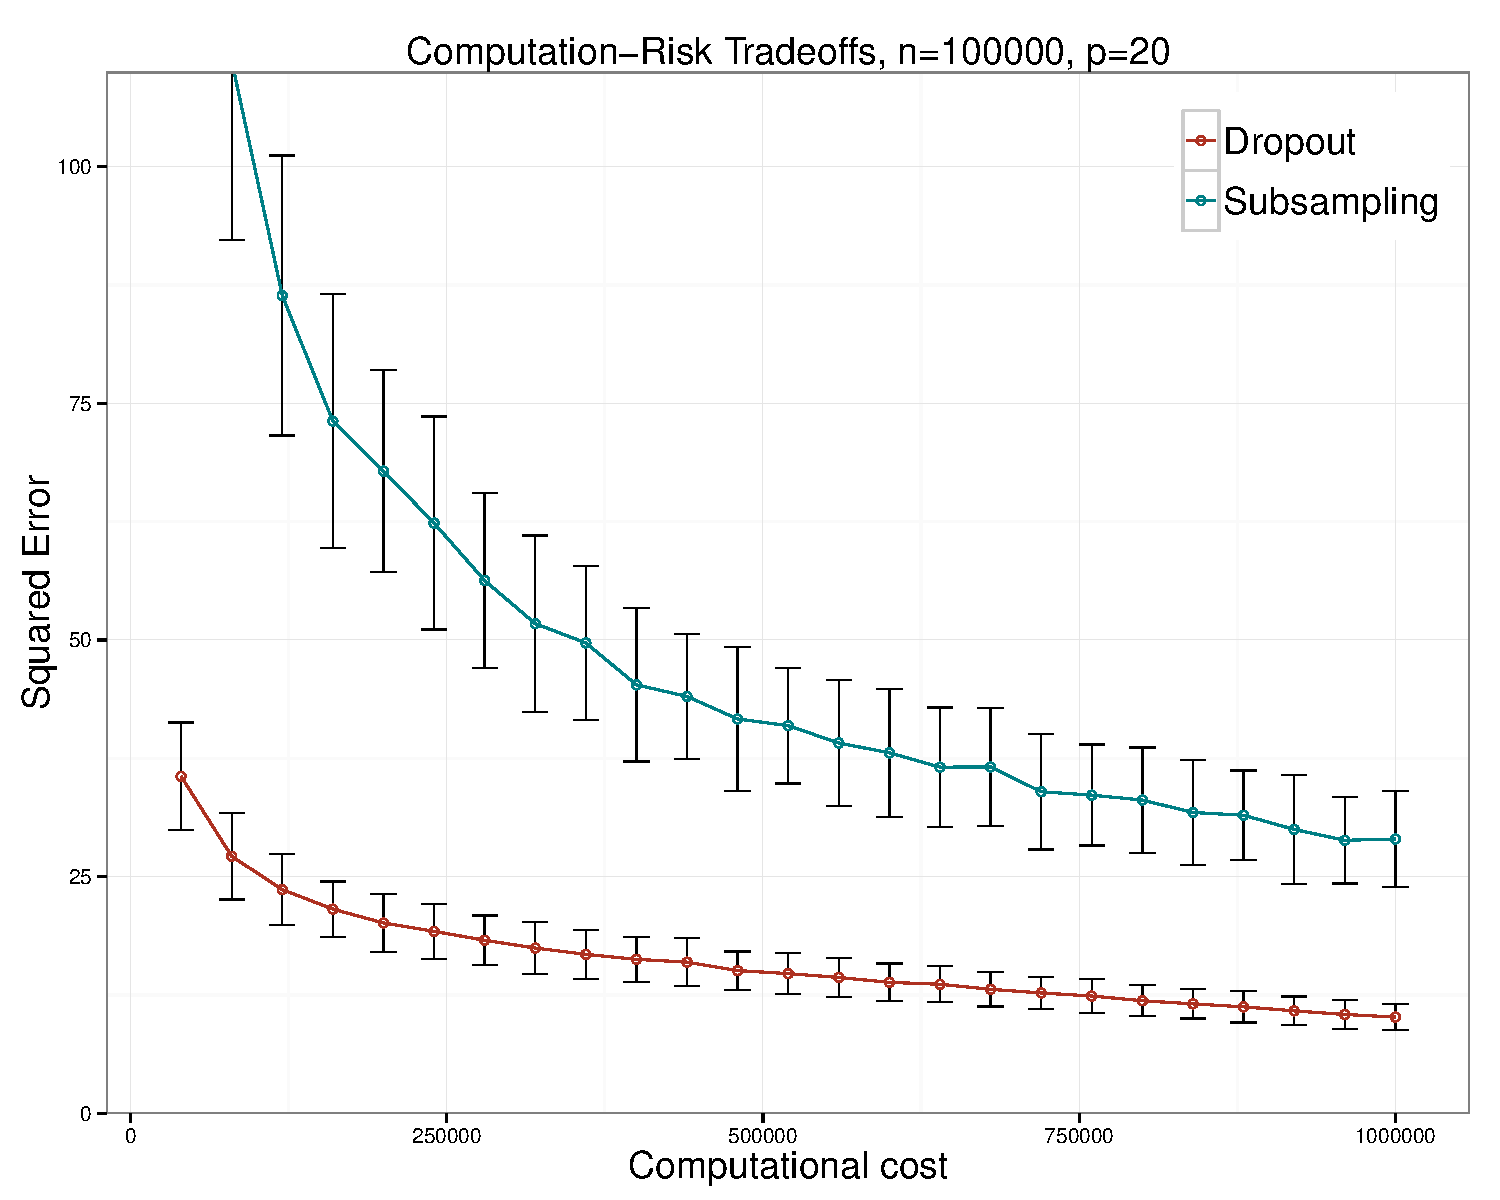
\includegraphics[width=.48\textwidth]{figs/dropout-subsample-n100000-p20-T100.pdf} &
\hskip-10pt
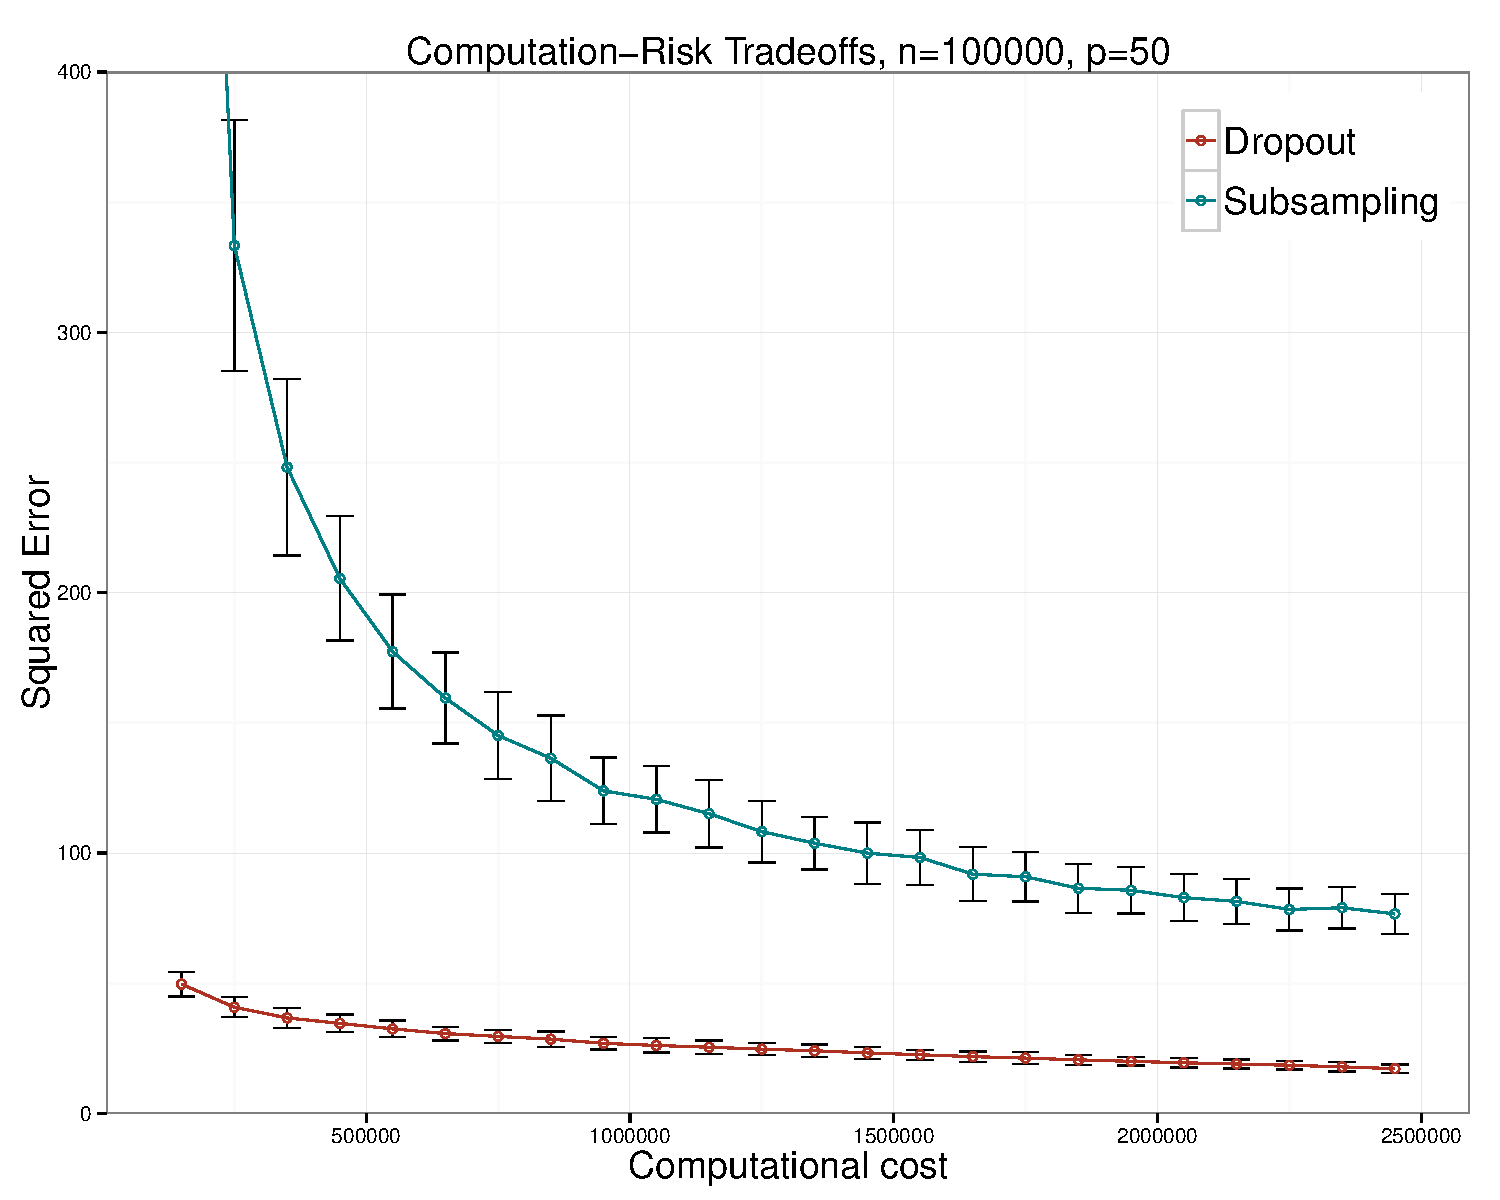
\includegraphics[width=.48\textwidth]{figs/dropout-subsample-n100000-p50-T100.pdf}
\end{tabular}
\end{center}
\caption{Comparision of subsampling to the dropout method for making
  computation-risk tradeoffs.  Two simulations are run, for $p=10$ and
  $p=20$ variables.  Subsampling with different subsample sizes $m$ is
  compared to the dropout with different dropout rates $\theta$.  The
  computational costs are measured by the theoretical bounds $O(mp^2 +
  p^3)$ for subsampling and $O(n\|\theta\|_1 + p^3)$ for the dropout,
  solved with subspace embedding. As $p$ increases, so does the
  relative advantage of the dropout.}
\label{fig:doss}
\end{figure}






\section{Subspace Embedding Algorithms}
\label{sec:subspaceembedding}



\section{Risk Analysis of Dropout Linear Regression}
\label{sec:droprisk}






\clearpage


\newpage
%\input{appendix}
%\newpage
%\input{notes}


\section*{Acknowledgements}
Research supported in part by NSF grants IIS-1116730, 
AFOSR grant FA9550-09-1-0373, ONR grant
N000141210762, and an Amazon AWS in Education Machine Learning
Research grant.


\bibliographystyle{imsart-nameyear}
\bibliography{graddrop}


\end{document}
